\documentclass{beamer}

\usepackage[francais]{babel}
\usepackage[utf8]{inputenc}  
\usepackage[T1]{fontenc}
\usetheme{Warsaw}

\title{Qt 2 : Qt Designer}

\author{Raihauti Teiki \and Minko Imrhan}

\institute[Université de Montpellier]

\date{20 Mars 2013}

\subject{Theoretical Computer Science}

\titlegraphic{
\includegraphics[width=2cm]{logo}
}

\AtBeginSubsection[]
{
  \begin{frame}<beamer>{Sommaire}
    \tableofcontents[currentsection,currentsubsection]
  \end{frame}
}

\begin{document}

\begin{frame}
  \titlepage
\end{frame}

\begin{frame}{Sommaire}
  \tableofcontents
\end{frame}


\section{Introduction}

\subsection{Qt}

\begin{frame}{Qt c'est quoi ?}
  \begin{itemize}
    \item {
        Qt est une API développée en C++ par QT Development Frameworks.
    \pause
    }
    \item {
        Qt permet principalement de modéliser des interfaces graphiques ou des widgets.
    \pause
    }
    \item {
        Cependant elle permet aussi d'accéder à des données ou à des connexions réseau.
    \pause
    }
    \item {
        Qt est multi-plateforme
    }
    \end{itemize}
\end{frame}


\subsection{Histoire de Qt}

\begin{frame}{Qt 1}
  \begin{itemize}
    \item {
        Le 26 mai 1995 est annoncée la première version publique de Qt. Le 24 septembre 1996, la version 1.0 est publiée.
    \pause
    }
    \item {
        Le projet KDE est lancé en 1997 et utilise Qt comme bibliothèque de base.
    \pause
    }
    \item {
        Le fait qu'un tel projet utilise Qt a permis au framework d'avoir une très bonne publicité et plusieurs versions apparaissent...
    }
    \end{itemize}
\end{frame}

\begin{frame}{Qt 2}
  \begin{itemize}
    \item {
        La seconde version majeure de Qt est publiée en juin 1999 et est une version pour les systèmes embarqués. Elle est connue sous le nom de Qtopia en 2000.
    \pause
    }
    \item {
         Cette dernière version est conçue pour Linux et utilise directement son framebuffer, sans passer par le système de fenêtrage X11.
    }
    \end{itemize}
\end{frame}

\begin{frame}{Qt 4}
  \begin{itemize}
    \item {
        La quatrième version de Qt permet l'apparition de modules tels que : 
    }
    
    \begin{description}[style=nextline]
        \item[QtGui] pour les composants graphiques
        \item[QtNetwork] pour la programmation réseau
        \item[QtSql] pour l'utilisation de base de données SQL
    \end{description} \pause

    \item {
        Et beaucoup d'autres modules dont celui qui nous intéresse : \textbf{Qt Designer}
    }
    \end{itemize}
\end{frame}


\subsection{Qt Designer}

\begin{frame}{Qt Designer}
  \begin{itemize}
    \item {
        Qt Designer est l'outil Qt permettant la conception et la construction d'interfaces graphiques avec Qt Widgets.
    \pause
   }
    \item{
        Lors de la compilation elles seront automatiquement reconverties en c++ et donc utilisables comme des classes normales.
    }
    
    \end{itemize}
\end{frame}
    
\begin{frame}{Qt Designer}
  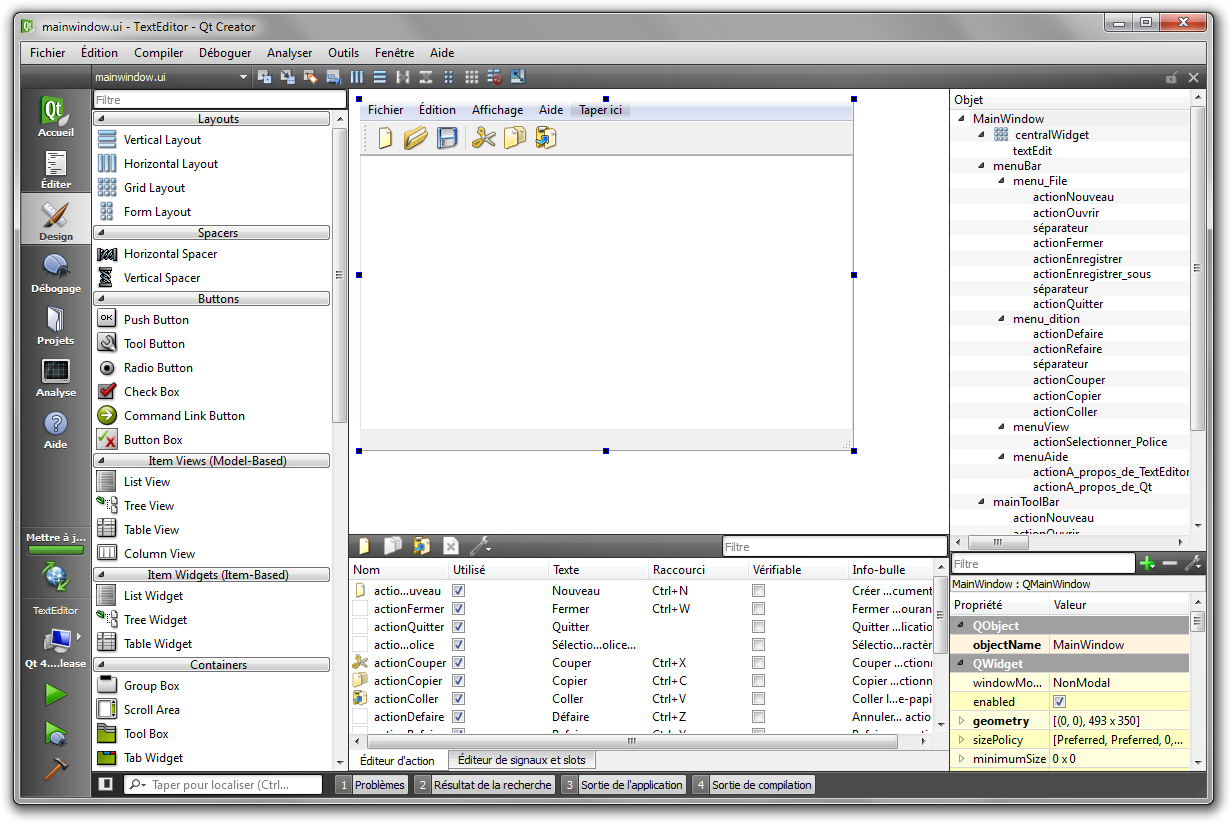
\includegraphics[width=10cm]{Qt-Designer}
\end{frame}   
   
\begin{frame}{Qt Designer}
  \begin{itemize}  
    \item {   
        Qt Designer permet aussi de modifier les propriétés des widgets, d'utiliser des layouts et d'effectuer la connexion entre signaux et slots.
    }
    \pause
    
    \item {
        Il utilise le mécanisme des signaux et des slots de Qt. Ce qui permet de facilement s'occuper des éléments graphiques.
    \pause
    }
    \item {
        Toutes les propriétés définies dans Qt Designer peuvent être modifiées dynamiquement dans le code. 
    }
    \end{itemize}
\end{frame}


\subsection{Précisions}

\begin{frame}{Précisions}
  \begin{itemize}
    \item {
        Qt est supportée par Mac depuis la version 3.0.
    }
    \item {
        La dernière version actuelle de Qt est la 5.0.
    }
    \item {
        Qt est utilisée par plusieurs grands groupes comme Google ou la NASA.
    }
    \item {
        Qt souvent prononcé Q.T mais se dit en fait "cute".
    }
    \end{itemize}
\end{frame}


\section{Utilisation de Qt Designer}

\subsection{Type de Fenêtre}

\begin{frame}{Type de Fenêtre}
    \begin{itemize}
        \item {
        Commencez d'abord par créer un projet 
        }
    \item {
        Lorsque vous demandez à créer une fenêtre, on vous propose de choisir le type de fenêtre.
    }
    \begin{description}[style=nextline]
        \item[Dialogs] fenêtre de types QDialog
        \item[MainWindow] pour gerer des menus et des barres d'outils
        \item[Widget] fenêtre de type QWidget
    \end{description} 
    \end{itemize}
\end{frame}
    
\begin{frame}{Type de Fenêtre}
    \includegraphics<1>[width=10cm]{fenetre.png}
\end{frame}

\subsection{Interface}

\begin{frame}{Interface}
    \includegraphics<1>[width=9cm]{interface.png}
\end{frame}
\begin{frame}{Interface}
\begin{itemize}
    \item {Au centre de Qt Designer, vous avez la fenêtre que vous êtes en train de dessiner.}
    \item{La Barre d'outils qui contient différent modes d'édition}
    \begin{description}[style=nextline]
        \item[Editer les Widgets] insérer des widgets sur la fenêtre et de modifier leurs propriétés.
        \item[Éditer signaux/slot] créer des connexions entre les signaux et les slots de vos widgets.
        \item[Éditer l'ordre des onglets] ermet de modifier l'ordre de tabulation entre les champs de la fenêtre
    \end{description}
\end{itemize}
    
\end{frame}
\begin{frame}{Interface}
\begin{itemize}
    \item {Widget Box : ce dock vous donne la possibilité de sélectionner un widget à placer sur la fenêtre. (situé à gauche)}
    \item{Property Editor : lorsqu'un widget est sélectionné sur la fenêtre principale, vous pouvez éditer ses propriétés. (en bas à droite)}
    \item{Object Inspector : affiche la liste des widgets placés sur la fenêtre. (en haut à droite)}
    \item{Éditeur de signaux/slots et éditeur d'action. (en bas)}
\end{itemize}
    
\end{frame}

\section{Conclusion}

\subsection{Conclusion}

\begin{frame}{Conclusion}
  \begin{itemize}
  \item
    \alert{Qt Designer} permet principalement de créer des fenêtres de manières visuelles.
  \item
    L'une des \alert{forces} est qu'il permet de \alert{ne pas} avoir à \alert{écrire des pavés de lignes de codes}.
  \item
  C'est un outil  \alert{complexe, mais intuitif}
  \end{itemize}
\end{frame}



% All of the following is optional and typically not needed. 
\appendix
\section<presentation>*{\appendixname}
\subsection<presentation>*{Pour plus d'informations}

\begin{frame}[allowframebreaks]
  \frametitle<presentation>{Pour plus d'informations}
    
  \begin{thebibliography}{10}
    
  \beamertemplatebookbibitems
  % Start with overview books.

  \bibitem{Jasmin2006}
    J. Blanchette and M. Summerfield
    \newblock {\em Qt4 et C++ : Programmation d'interfaces GUI}.
    \newblock CampusPress, 2007.
 
    
  \beamertemplatearticlebibitems
  % Followed by interesting articles. Keep the list short. 

  \bibitem{QT2000}
        The Qt Company
    \newblock http://doc.qt.io/qt-5/qtdesigner-manual.html
  \end{thebibliography}
\end{frame}
\begin{frame}{FIN}

\center {PLACE À LA DÉMO}
    
\end{frame}

\end{document}


